\section{Resultados}

Todo el código mostrado anteriormente carece de significado su su operación no es mostrada. A continuación veremos 3 quintuplas en operación con nuestro algoritmo y dadas algunas cadenas de entrada, veremos el resultado que producen:

\subsection{Autómata Finito 1}

El siguiente autómata finito dado por la quintupla (2):

\begin{itemize}
\item Q: $\{$0, 1, 2, 3$\}$
\item $\Sigma$: $\{$a, b$\}$
\item $q_{0}$: 0
\item F: $\{$2$\}$
\item $\alpha$: $\{$(0,a,0), (0,b,0), (0,a,1), (1,b,2), (1,a,3), (2,a,3), (2,b,3), (3,a,3), (3,b,3)$\}$
\end{itemize}

Produce la siguiente salida en nuestro programa con la cadena de entrada \textbf{aaab}:

\begin{figure}[H]
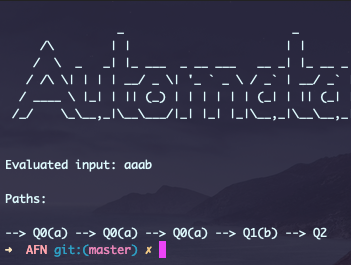
\includegraphics[width = 16.5cm, height = 8cm]{afn-1-aaab.png}
\centering \linebreak \linebreak {\small Figure 1.0: Caminos que la cadena \textbf{aaab} puede seguir para llegar a su estado de aceptación.}
\end{figure} 

Produce la siguiente salida en nuestro programa con la cadena de entrada \textbf{ababab}:

\begin{figure}[H]
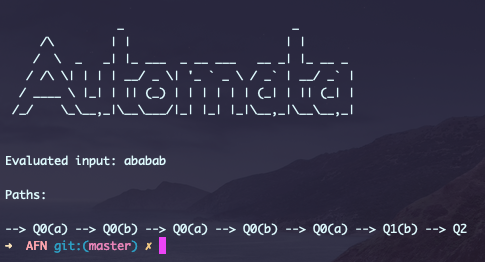
\includegraphics[width = 16.5cm, height = 8cm]{afn-1-ababab.png}
\centering \linebreak \linebreak {\small Figure 1.1: Caminos que la cadena \textbf{ababab} puede seguir para llegar a su estado de aceptación.}
\end{figure} 

\subsection{Autómata Finito 2}

El siguiente autómata finito dado por la quintupla (2):

\begin{itemize}
\item Q: $\{$1, 2, 3, 4, 5, 6$\}$
\item $\Sigma$: $\{$a, b$\}$
\item $q_{0}$: 1
\item F: $\{$3, 4, 5$\}$
\item $\alpha$: $\{$(1,a,2), (1,a,5), (1,b,4), (2,a,2), (2,b,3), (3,a,6), (3,b,6), (4,a,6), (4,b,6), (5,a,6), (5,b,5), (6,a,6), (6,b,6)$\}$
\end{itemize}

Produce la siguiente salida en nuestro programa con la cadena de entrada \textbf{aaab}:

\begin{figure}[H]
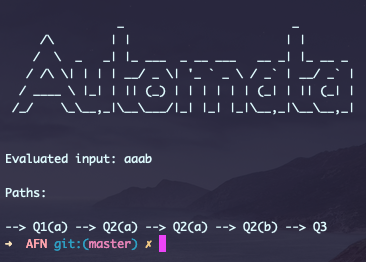
\includegraphics[width = 16.5cm, height = 8cm]{afn-2-aaab.png}
\centering \linebreak \linebreak {\small Figure 2.0: Caminos que la cadena \textbf{aaab} puede seguir para llegar a su estado de aceptación.}
\end{figure} 

Produce la siguiente salida en nuestro programa con la cadena de entrada \textbf{ab}:

\begin{figure}[H]
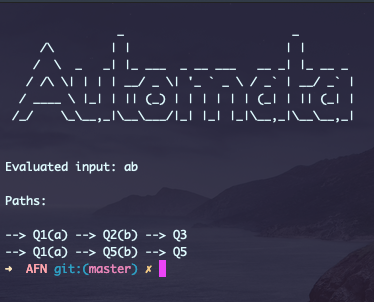
\includegraphics[width = 16.5cm, height = 8cm]{afn-2-ab.png}
\centering \linebreak \linebreak {\small Figure 2.1: Caminos que la cadena \textbf{ab} puede seguir para llegar a su estado de aceptación.}
\end{figure} 

Produce la siguiente salida en nuestro programa con la cadena de entrada \textbf{abab}:

\begin{figure}[H]
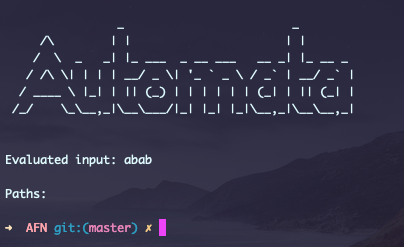
\includegraphics[width = 16.5cm, height = 8cm]{afn-2-abab.png}
\centering \linebreak \linebreak {\small Figure 2.2: Caminos que la cadena \textbf{abab} puede seguir para llegar a su estado de aceptación.}
\end{figure} 

\subsection{Autómata Finito 3}

El siguiente autómata finito dado por la quintupla (2):

\begin{itemize}
\item Q: $\{$0, 1, 2, 3, 4$\}$
\item $\Sigma$: $\{$a, +, -, .$\}$
\item $q_{0}$: 0
\item F: $\{$3$\}$
\item $\alpha$: $\{$(0,+,1), (0,-,1), (0,.,2), (0,a,4), (1,.,2), (1,a,1), (1,a,4), (2,a,3), (3,a,3), (4,.,3)$\}$
\end{itemize}

Produce la siguiente salida en nuestro programa con la cadena de entrada \textbf{a.aa}:

\begin{figure}[H]
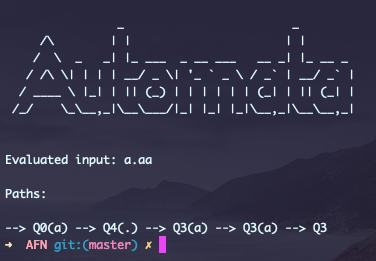
\includegraphics[width = 16.5cm, height = 8cm]{afn-3-1.png}
\centering \linebreak \linebreak {\small Figure 3.0: Caminos que la cadena \textbf{a.aa} puede seguir para llegar a su estado de aceptación.}
\end{figure} 

Produce la siguiente salida en nuestro programa con la cadena de entrada \textbf{+a.a}:

\begin{figure}[H]
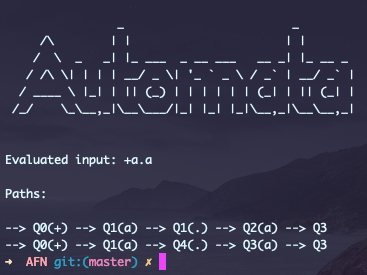
\includegraphics[width = 16.5cm, height = 8cm]{afn-3-2.png}
\centering \linebreak \linebreak {\small Figure 3.1: Caminos que la cadena \textbf{+a.a} puede seguir para llegar a su estado de aceptación.}
\end{figure} 

Produce la siguiente salida en nuestro programa con la cadena de entrada \textbf{+aa.aa}:

\begin{figure}[H]
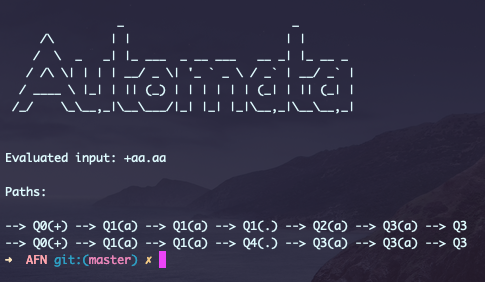
\includegraphics[width = 16.5cm, height = 8cm]{afn-3-3.png}
\centering \linebreak \linebreak {\small Figure 3.2: Caminos que la cadena \textbf{+aa.aa} puede seguir para llegar a su estado de aceptación.}
\end{figure} 